\subsection{Performance}
\label{sec:eval-dedup}


\begin{table}[h!]
	%\centering
	%\tiny 
	\scriptsize
	\caption{Workload parameters.}
	\begin{tabular}{| c | c | c | c | c | c | c| c |} 
		\hline
	Trace    &   \#GET L & \#GET M & \#PUT L & \#PUT M & \#Uniq L & \#Uniq M \\ 
		\hline\hline
		Dal    &  2867  & 2000   & 124  & 9     & 1278 & 88      \\ 
		\hline
		Fra     &  1602  & 3278   & 111  & 9     & 420 & 43     \\
		\hline
		Lon    &  924    & 3972   & 98  & 6      & 698 & 88    \\
		\hline 
		Syd      &  1310   & 3653   & 35 & 2     & 154 & 18      \\  
		\hline
	\end{tabular}

\label{tab:eval-overall}
\end{table}


%\begin{table}[h!]
%	%\centering
%	\scriptsize 
%	\caption{Testing Dataset.}
%	\begin{tabular}{| c | c | c | c | c | } 
%		\hline
%		Trace  (GB)  &   Dataset  & Data transferred  & GET L size  & PUT L size  \\ 
%		\hline\hline
%		Dal   & 20  & 37 & 35 & 2    \\ 
%		\hline
%		Fra     & 6  & 16 & 14 & 2   \\
%		\hline
%		Lon    &10   &  14 &12  & 2      \\
%		\hline 
%		Syd      &  2  &  9 & 8 & 1      \\  
%		\hline
%	\end{tabular}
%	
%	\label{tab:eval-dataset}
%\end{table}


%\begin{figure}[t]
%	\centering
%	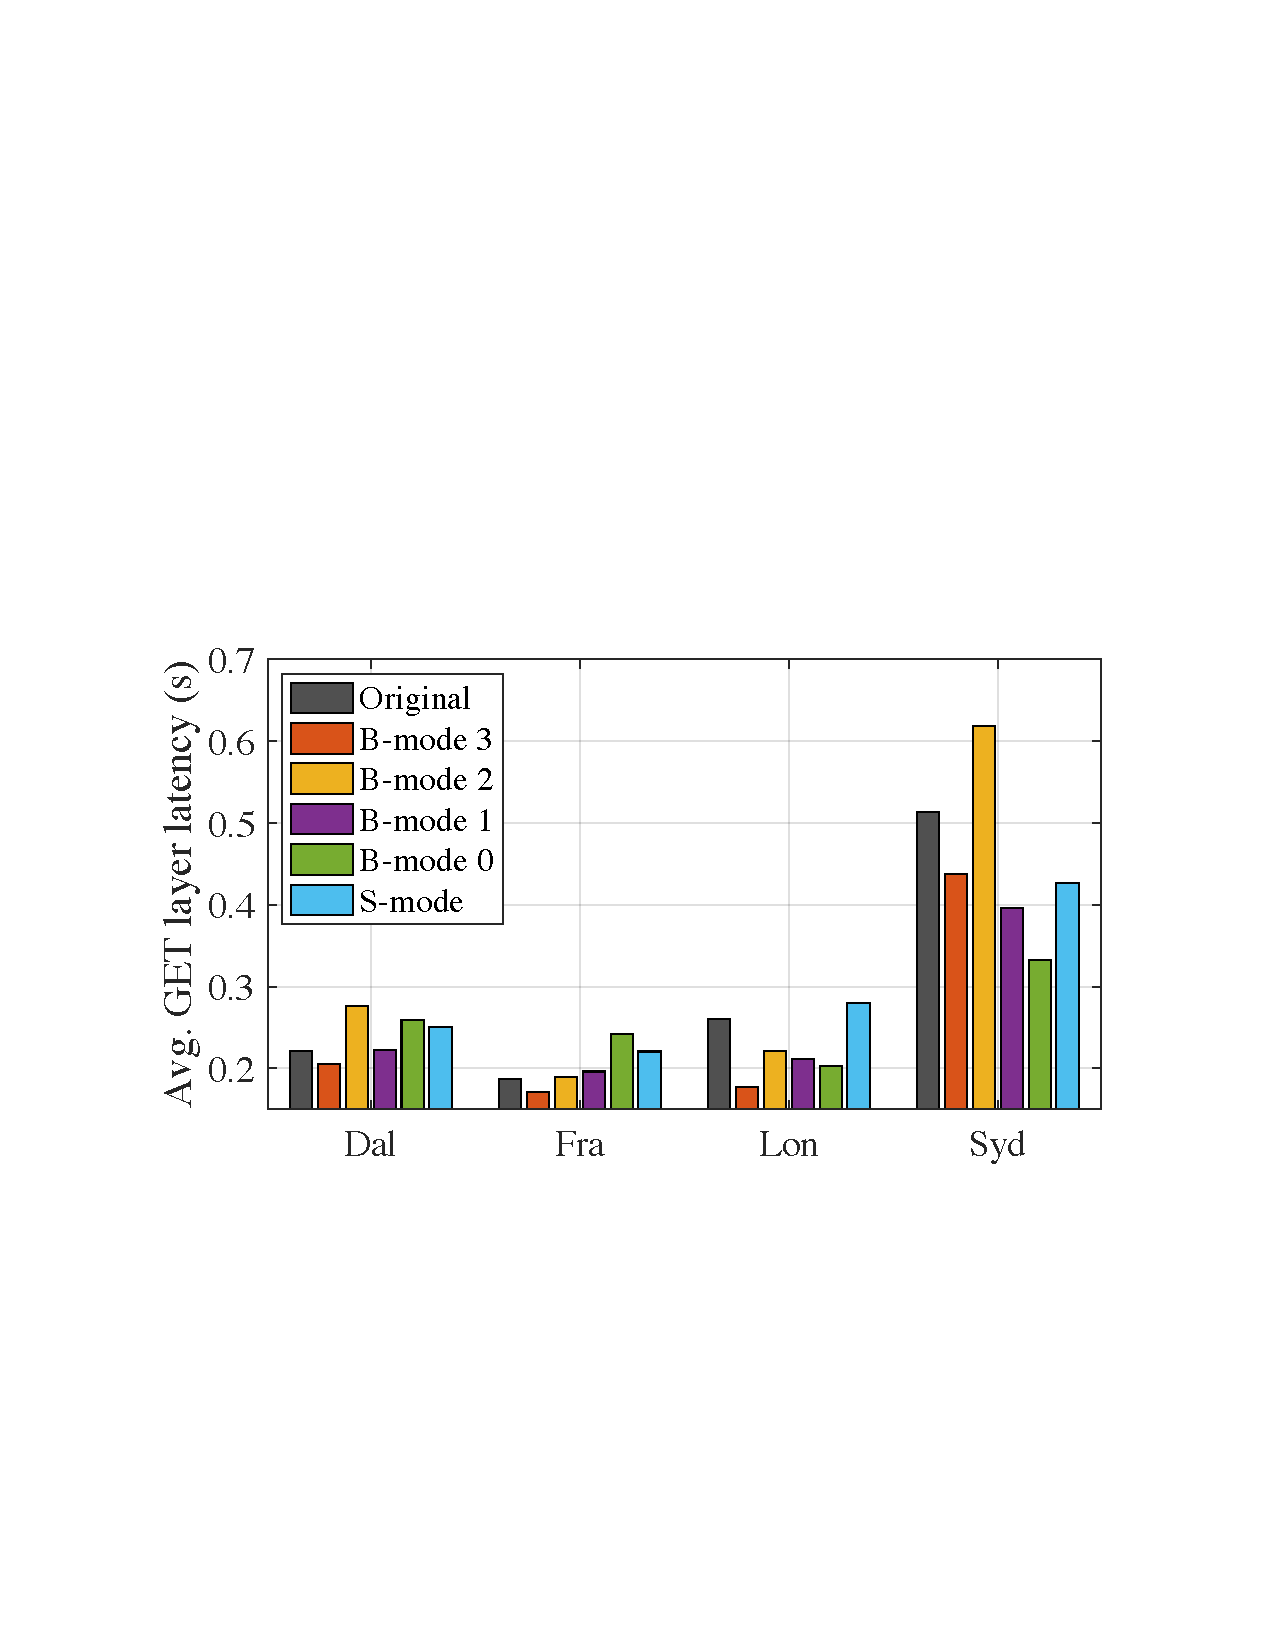
\includegraphics[width=0.45\textwidth]{graphs/get-layer-latency.pdf}
%	\caption{GET layer latency across different workloads from different schemes.}
%	%	\vspace{-3pt}
%	\label{fig:getlayerlatency}
%	
%\end{figure}



\subsubsection{Overall performance}


\subsubsection{Breakdown performance}


\subsubsection{Performance Comparison}


\subsubsection{Performance with different parameters}

\paragraph{Layer size impact}

\paragraph{Cache parameter impact}

\paragraph{Registry cluster size impact}

\paragraph{Repull threshold}

\paragraph{Compression level}
%\section{Deduplication performance}
%\label{sec:Evaluation}
%
%%Our two-tier heterogeneous cache in the registry can improve the performance of the entire system
%%by hiding the long latency imposed by the backend dedup system.
%%Next, we present the preliminary evaluation of our user access history-based cache algorithm
%%and the space efficiency of file cache.
%
%\vspace{-6pt}
%\paragraph{Cache hit ratio.}
%
%We simulate our user-access-history-based cache and 
%replay the \texttt{dal} workload~\cite{dockerworkload} to measure the hit ratio. We set the cache size to be $20$\% of the data ingress for \texttt{dal}. We set $10$\% of the cache for buffering incoming \texttt{put} layer requests, and 
%the rest for caching prefetched layer slices from backend servers. 
%Note that in this evaluation, the cache only contains the layer buffer without the file cache.
%%as shown in Figure~\ref{fig:hitratio}.
%%Our algorithm exhibits an enhanced cache performance, with a high hit ratio
%%up to 0.96.
%Figure~\ref{fig:hitratio} shows the results. We observe a significant increase in the hit ratio, $74$\% to $95$\% as the duration threshold grows from $1$ to $10$ minutes. This is because prefetched layers are kept in the cache for more time.
%The hit ratio stablizes at $96$\% as the duration threshold increases from $15$ to $20$ minutes.
%%Therefore,
%%the highest hit ratio of our algorithm is around 0.96,
%%and there are 0.4 of layers that are miss because 
%%some users \emph{re-pull} the layers after they pull the same layers.
%The layers responsible for the $4$\% miss rate are the ones being
%\emph{re-pulled} by the same user.
%%We also see that 74\% of users can finish their \texttt{pull} layer request
%%within a minute and 
%%around 89\% of users can finished their \texttt{pull} layer request with less than 5 min. 
%%We also see that the response time to \texttt{pull} layer requests is within $1$ minute for 74\% of users, and it is less than $5$ minutes for 89\% of users.
%%Since we buffer layers upon a \texttt{push} layer request and prefetch layer {\em slices} from the backend servers, 
%%we compare the hits on prefetched layer {\em slices} and the hits on buffered layers.
%We see that, across different duration thresholds, 
%the hits upon buffering newly put requests (denoted as buffering hit ratio) is very low,
%confirming that it takes a long time for a recently \emph{pushed} layer to be pulled.
%We also observe a $22$\% average cache utilization. 
%That is because our algorithm is based on users demand 
%so it adapts to workload changes.
%%This trend is perfectly fit in our two-tier heterogeneous cache
%%and the evaluation results can guide us to carefully choose 
%%layer buffer size and file cache size.
%%
%%In terms of file count, it increases from \textbf{3.6$\times$} to \textbf{31.5$\times$} while
%%in terms of capacity, it increases from \textbf{1.9$\times$} to
%%\textbf{6.9$\times$} as the layer dataset grows from 1000 to 1.7 million layers.
%%%
%%This confirms the high potential for file-level deduplication in large-scale
%%Docker registry deployments.
%
%\vspace{-6pt}
%\paragraph{Space efficiency.}
%%As shown in Figure~\ref{xxx},
%%we compare the cache hit ratio of LRU, Prefetch~\cite{xxxx}, and our 
%%user-based cache replacement algorithm by replaying three IBM container registry workloads~\cite{dockerworkload}.
%%Our user-based cache exhibits an enhanced cache performance, with hit ratio improvements ranging from 
%%0.2 to 0.3 for all the three workloads compared to LRU.
%We analyze the space efficiency of the file cache compared to a cache that naively stores
%compressed layers.
%%for an increasing number of files stored in the file cache 
%%(see Figure~\ref{fig:dedup-ratio-growth}).
%%
%%Figure~\ref{fig:dedup-ratio-growth} shows the deduplication ratio growth over the layer dataset size.
%%
%In Figure~\ref{fig:cacheefficiency}, the x-axis values correspond to the sizes of $4$ random samples drawn from the whole dataset and the size of the dataset in terms of capacity and layer count.
%For a traditional cache, the compressed layer tarballs will be kept as is.
%While \sysname will store \emph{deduped} layers. 
%%unique files in the file cache.
%The y-axis shows how many more \emph{deduped} layers can fit in our file cache compared to naively storing compressed layer tarballs.
%For the first two samples of the dataset, with size less than $20$~GB, 
%there is no benefit to \emph{dedup} layers 
%because the deduplication ratio is very low.
%However, when the dataset size is $3$~TB, we can store $56\%$ more \emph{deduped} layers' unique files in file cache.
%The number of extra \emph{deduped} layers that can fit in the file cache increases almost linearly with the size of the layer dataset.
%%the bigger the dataset, the more deduped layers that can fit in the file cache.
%%The number of extra layers increases almost linearly with the layer dataset size.
%%In this case, there is a high potential for file cache when the cache size is big.
%This verifies the benefit of the file cache when the cache size is large, which should be carefully selected to realize significant space savings.


%In this experiment, we show how many more layers can be stored in the file cache 
%after decompression and file-level deduplication.
%Figure~\ref{xxxx} shows the growth of deduplication ratio with different dataset sizes.


%We evaluated \sysname's performance improvement over traditional 

%%While \sysname\ can effectively eliminate redundant files in the
%%Docker registry, it introduces overhead which can reduce the
%%registry's performance.
%%
%%The overheads can be classified in two categories: 1)~\emph{background
%%overhead} caused by the computation and I/O that is performed during layer
%%deduplication; and 2)~\emph{foreground overhead} from extra processing on the
%%critical path of a pull request.
%%\begin{figure}
	\centering
	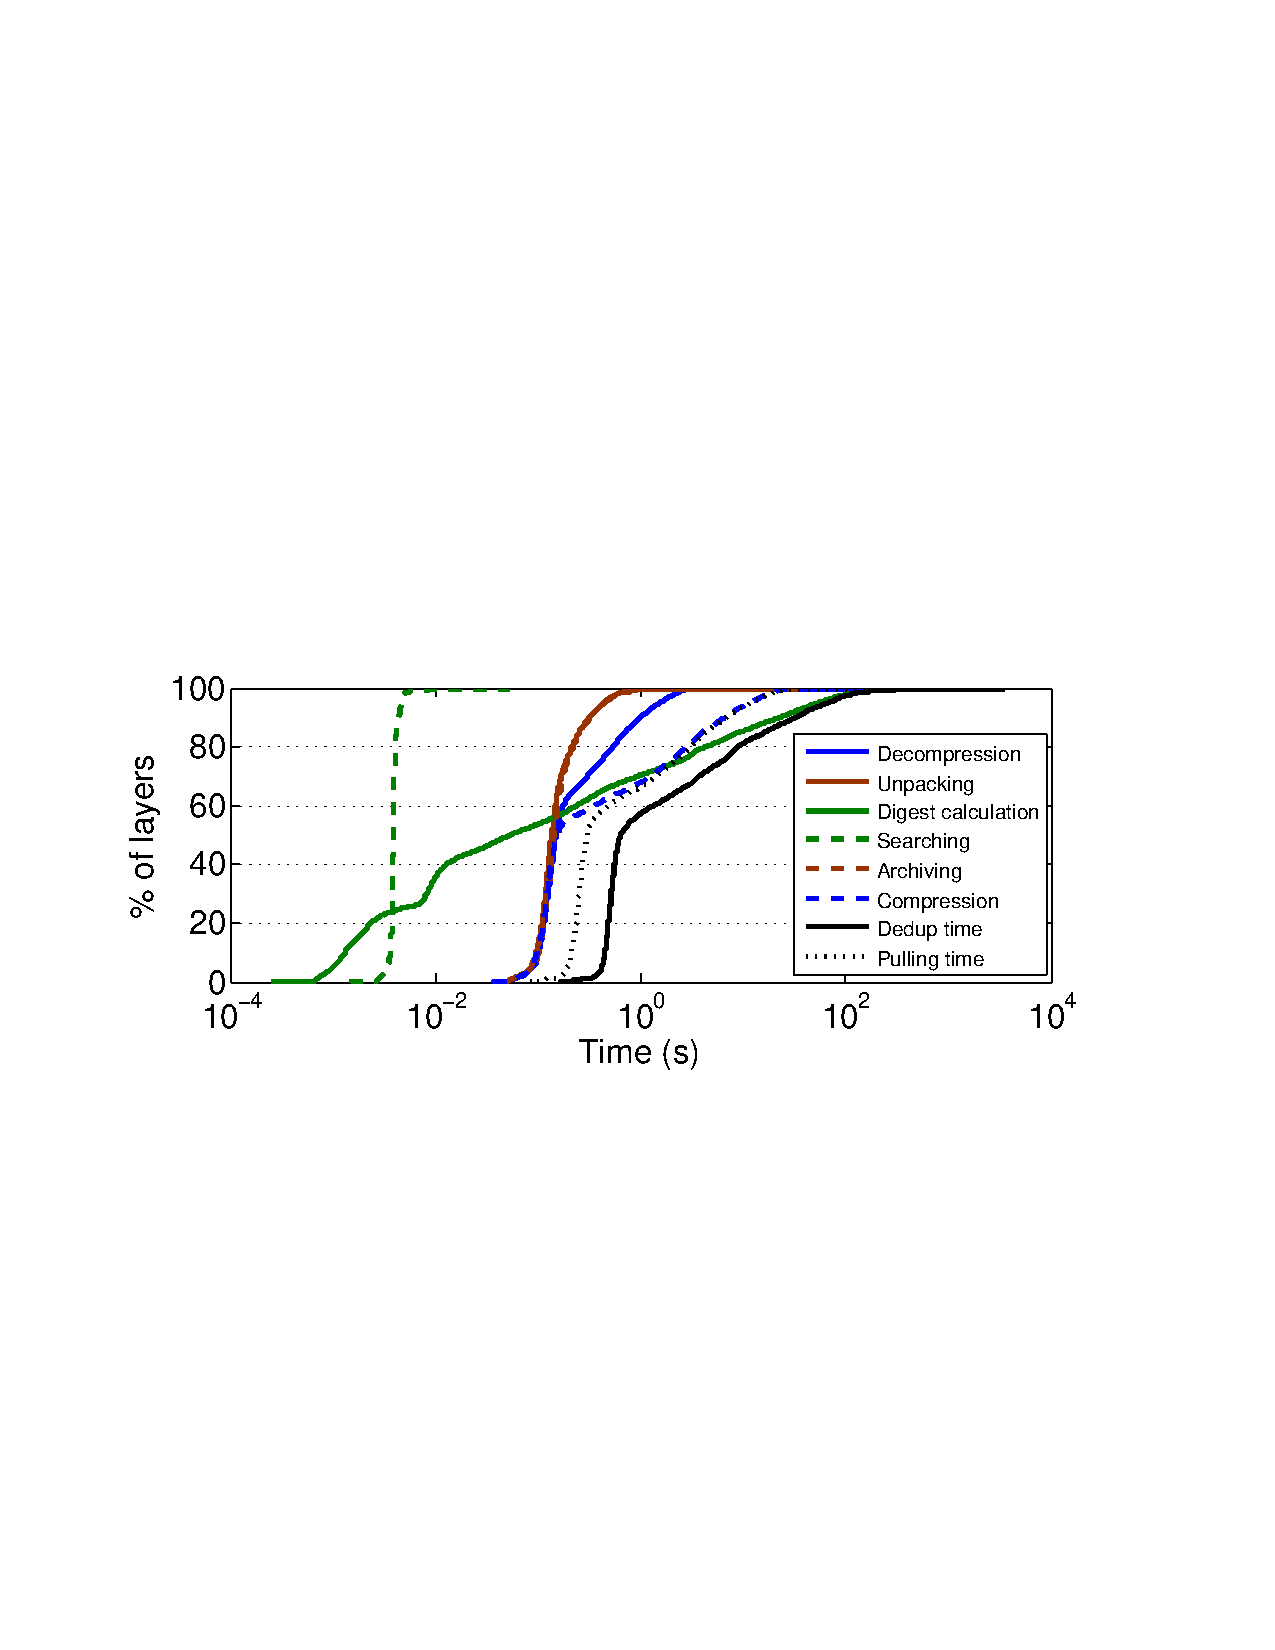
\includegraphics[width=0.5\textwidth]{graphs/res-time.pdf}
	\caption{Off-line file-level deduplication run time.}
	\label{fig:dedup-res}
\end{figure}

%
%
%%\paragraph{Hit ratios}
%%
%%\paragraph{Hit ratios with prefetching}
%%
%%%\subsection{} % what are the cost for a naive file-level deduplication
%%
%%\paragraph{Restoring performance breakdown}
%%
%%\paragraph{Simulation}
%%
%%To analyze the impact of file-level deduplication on the registry performance,
%%we conduct a preliminary simulation-based study of \sysname.
%%
%%Based on the simulation results, we estimated the overhead of \sysname\ on
%%\texttt{push} and \texttt{pull} layer request latencies.
%%
%%We then provide different suggestions on how the Docker registry can mitigate
%%the deduplication overhead.
%%
%%%%%%%%%%%%%%%%%%%%%%%%%%%%%%%%%%%%%%%%%%%%%%%%%%%%%%%%%%%%%%%%%%%%%%%%%%%%%
%%
%%
%Our simulation
%approximates several of \sysname's steps as described in Section~\ref{sec:design}.
%%
%First, a layer from our dataset is copied to a RAM disk. 
%%
%%
%%Note that there is no foreground pull or push requests since the simulation is \emph{off-line}.
%%
%The layer is then decompressed, unpacked, and the fingerprints of all files
%are computed using the MD5 hash function~\cite{MD5}.
%%
%The simulation searches the fingerprint index for duplicates,
%and, if the file has not been stored previously, it records the
%file's fingerprint in the index.
%%
%%To map a layer to its containing files, we create the layer recipe and add it
%%to a \emph{layer-to-file table}.
%%
%%The simulator then creates a file recipe.
%%
%%For each file in a layer, a layer digest
%%to its containing file content digest mapping record is also created 
%%
%%The \emph{layer-to-file table} also
%%records the file path within each layer associated with each file.
%%
%At this point our simulation does not include
%the latency of storing unique files.
%%
%To simulate the layer reconstruction during a \texttt{pull} request,
%we archive and compress the corresponding files.
%%
%%Only unique files are maintained in RAM
%%disk while the redundant copies are removed.
%%
%
%The simulator is implemented in 600 lines of Python code
%and our setup is a one-node Docker registry on a machine with 32~cores and 64\,GB of RAM.
%%
%To speed up the experiments and fit the required data in RAM
%we use 50\% of all layers and exclude the ones larger than 50\,MB.
%%
%We process 60 layers in parallel using 60 threads.
%%
%The entire simulation took 3.5 days to finish.
%%
%%The overall runtime is about 3.5 days.
%
%Figure~\ref{fig:dedup-res} shows the CDF for each sub-operation of
%\sysname.
%%
%Unpacking, Decompression, Digest Calculation, and Searching 
%are part of
%the deduplication process and together make up the Dedup time.
%%
%%\VT{@Nannan, in Figure ~\ref{fig:dedup-res} can you reorder the lines in the
%%legend so that the Searching goes after Digest calculation?}\NZ{addressed}
%%
%Searching, Archiving, and Compression
%simulate the processing for a \texttt{pull}
%request and form the Pulling time.
%%
%
%%\LR{What was the overall runtime for processing 0.9 million layers?}\NZ{addressed}
%%
%%\alicomment{How are we saving the location
%%of each file in the layer? It is not clear from the following sentences.}
%%\NZ{addressed}
%%
%%To improve searching performance, the
%%mapping table is stored in Hive database~\cite{xxx}. 
%%
%%\lrcomment{Why are we using Hive for this? It seems overkill to me, especially
%%for such small data. Even at scale, a KeyValue store would probably provide
%%better performance than clunky MapReduce-based DB.}
%%
%
%\paragraph{Push}
%
%\sysname\ does not directly impact the latency of \texttt{push} requests because
%deduplication is performed asynchronously.
%%ie the registry reliably stores a
%%copy of the layer as-is and then sends a response to the client.
%%
%The appropriate performance metric for \texttt{push} is the time it takes to deduplicate
%a single layer.
%%
%%Next, we look at the effects on \texttt{push} and \texttt{pull} latencies in
%%more detail.
%%
%%However, if there are intensive push requests while the registry is performing
%%deduplication, \sysname\ can still impact push latencies because it incurs
%%CPU, memory, and I/O overhead. %(similar to pull requests).
%%
%Looking at the breakdown of the deduplication time in
%Figure~\ref{fig:dedup-res}, we make several observations.
%
%First, the searching time is the smallest among all operations with 90\% of the
%searches completing in less than 4\,ms and a median of 3.9\,ms.
%%
%%The mapping table maintains 0.98 million layer-to-file digest mapping records. 
%%
%%\LR{Remove the following sentence? 1.7 million records is actually quite small
%%so even a single-node DB with one index is enough.}\NZ{addressed} Consider
%%that more than 1.7 million layers are stored in Docker hub and the number is
%%still increasing, it's better to choose a fast distributed database to provide
%%high searching performance and scalability.
%%
%Second, the calculation of digests spans a wide range from 5\,$\mu$s to almost
%125\,s.
%%
%%This is because the time mainly depends on the layer size, \ie the fewer and
%%smaller files a layer contains, the faster it is to compute all digests for
%%the layer.
%%
%%Typically, smaller layers contain a smaller number of smaller files, which
%%takes much less time to calculate their digests.
%%
%%While if the layer is bigger, the digest calculation overhead will be higher. 
%%
%90\% of digest calculation times are less than 27\,s while 50\% are
%less than 0.05\,s.
%%
%The diversity in the timing is caused by a high variety of layer sizes both in
%terms of storage space and file counts.
%%
%%Thus, we suggest that multiple-threading is needed to calculate the files'
%%digests simultaneously; 
%%
%%Fast CPUs as well as more powerful computing nodes are required to speed up
%%digest calculation.
%%
%Third, the run time for decompression and unpacking follows an identical
%distribution for around 60\% of the layers and is less than 150\,ms.
%%
%%Around 60\% of decompression and unpacking time are less than 0.15\,s. 
%%
%However, after that, the times diverge and decompression times increase faster
%compared to unpacking times.
%%
%%\VT{do we have some theory why?}
%%\NZ{decompressing the layers with bigger uncompressed size takes longer time.}
%%
%90\% of decompressions take less than 950\,ms while 90\% of packing time is less
%than 350ms.
%
%%Overall, we see that file digest calculation contributes a lot to the
%%overall deduplication latency especially when the layer size is big.  Moreover,
%%we see that the deduplication latency increases as the layer size grows.
%%
%Overall, we see that 90\% of file-level deduplication time is less than 35\,s
%per layer, while the average processing time for a single layer is 13.5\,s.
%%
%This means that our single-node deployment can process about 4.4\,layers/s on average
%(using 60 threads).
%%
%In the future we will work on further improving \sysname's deduplication throughput.
%%
%%In a large-scale registry deployment, this throughput can be improved
%%as more node are available to perform deduplication.
%%
%
%\paragraph{Pull} 
%
%From Figure~\ref{fig:dedup-res}
%we can see that 55\% of the layers have close compression and archiving
%times ranging from from 40\,ms to 150\,ms and both operations contribute equally
%to pulling latency.
%%
%%60\% of compression and archiving time are less than 0.15 s.
%%
%%While compression has the highest run time 80\% of compression time is less than 2.82~s. 
%%
%%\LR{Again, better to show the 90th percentile.}
%%\NZ{90\% of the compression time is less than 8\,s.}
%After that, the times diverge and compression times increase faster with an
%90\textsuperscript{th} percentile of 8\,s.
%%
%This is because compression times increase for larger layers and follow the distribution
%of layer sizes (see Figure~\ref{fig:layer-size-cdf}).
%%
%%80\textsuperscript{th} percentile of 2.82\,s.
%%
%Compression time makes up the major portion of the pull latency and is a
%bottleneck.
%%
%Overall, the average pull time is 2.3\,s.
%
%%
%%We see that archiving time and compression contributes equally to pulling
%%latency when their run time are lower than 0.15 s while compression time almost
%%equals to pulling latency when the compression time is greater than 0.15 s. 
